\chapter{Revisão Bibliográfica}

A propagação de modos normais (ondas planas) é um problema clássico em acústica e continua tendo importância significativa mediante ao advento de novas tecnologias relacionadas a sistemas de exaustão e sucção. Em geral, pode-se utilizar dois parâmetros para caracterizar o fenômeno da acústica interna de dutos:

\begin{itemize}
    \item a magnitude do coeficiente de reflexão $\|R\|$, razão entre as componentes refletida e incidente da onda no duto, a qual é dada por
    \begin{equation}
        R_{r}\simbolo{$R_{r}$}{Coeficiente de reflexão} =\frac{Z_{r} - Z_{0}}{Z_{r} + Z_{0}},
        \label{eq:R}
    \end{equation}
    sendo $Z_{r}$\simbolo{$Z_{r}$}{Impedância de radiação} a impedância de radiação e $Z_{0}$\simbolo{$Z_{0}$}{Impedância característica do meio} a impedância característica do meio;
    
    \item coeficiente de correção da terminação normalizado pelo raio do duto $l/a$ em que $a$ é o raio do duto. Tal parâmetro representa o comprimento acústico efetivo do duto. Em outras palavras, o fator $l$ é a quantidade adicional medida a partir da abertura do duto a qual deve propagar a onda incidente antes de ser refletida para o interior do duto com fase invertida. Tal coeficiente de correção da terminação $l$ é dado por
    \begin{equation}
        l = \frac{1}{k} \arctan\!\left(\frac{Z_{r}}{Z_{0} \, \mathrm{i}\simbolo{$i$}{Número imaginário}}\right)
        \label{eq:l}
    \end{equation}
    sendo $k$\simbolo{$k$}{Número de onda} o número de onda.
\end{itemize}

Em relação aos parâmetros discutidos acima, a solução exata para o problema de um duto não flangeado na ausência de escoamento foi proposta por \citeonline{levine1948radiation}. A solução assume que a espessura das paredes do duto são desprezíveis e o fluido é inviscido. A partir destas simplificações, as expressões exatas para $\|R\|$ e $l$ são obtidas utilizando-se a técnica de Wiener-Hopf.

Apesar da utilidade do modelo de Levine e Schwinger, em boa parte das aplicações práticas, dutos transportam escoamentos médios. Para tais circunstâncias, \citeonline{munt1990acoustic} propôs um modelo analítico exato, também baseado na técnica de Wiener-Hopf, em que se considera a presença de um escoamento subsônico no interior do duto. Considera-se nesse modelo as premissas de que o escoamento é uniforme, invíscido e que a camada cisalhante do jato é infinitamente fina. Além disso, o modelo considera a condição de Kutta na borda do duto para lidar com a singularidade da velocidade de partícula nesta região. As Figuras \ref{fig:comp1} e \ref{fig:comp2} apresentam as comparações entre casos com e sem escoamento para um duto não flangeado em termos de $\|R\|$ e $l/a$.

\begin{figure}[ht!]
\centering
  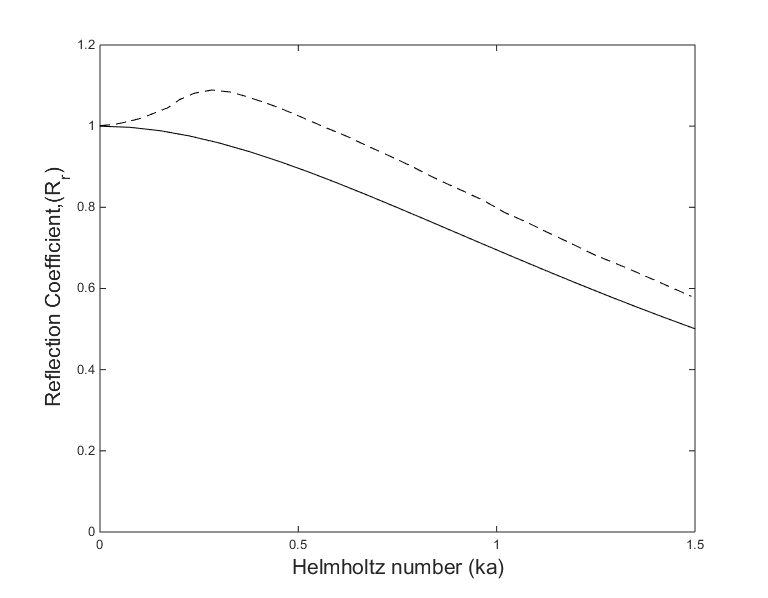
\includegraphics[width=.9\linewidth]{figuras/abs_r_comparacao.png}
  \caption[Magnitudes do coeficiente de reflexão $|R|$]{Resultados analíticos exatos para magnitude do coeficiente de reflexão $\|R\|$ ao final de um duto não flangeado. A linha contínua apresenta o resultado sem escoamento de \citeonline{levine1948radiation} e a linha tracejada apresenta o resultado com escoamento de Mach = 0,15 de \citeonline{munt1990acoustic}.}
  \label{fig:comp1}
\end{figure}

Como é mostrado na Figura \ref{fig:comp1}, a magnitude do coeficiente de reflexão $\|R\|$ aumenta consideravelmente na presença de um escoamento subsônico. Além disso, pode-se perceber que, em algumas frequências, $\|R\|$ torna-se maior do que a unidade, implicando que a amplitude da onda refletida torna-se maior do que a da onda incidente. Este fenômeno ocorre, sobretudo, pela transferência de energia cinética rotacional do escoamento para o campo acústico. Essa transferência de energia cinética ocorre sobretudo pelo desprendimento periódico de vórtices na borda do duto.

\begin{figure}[ht!]
\centering
  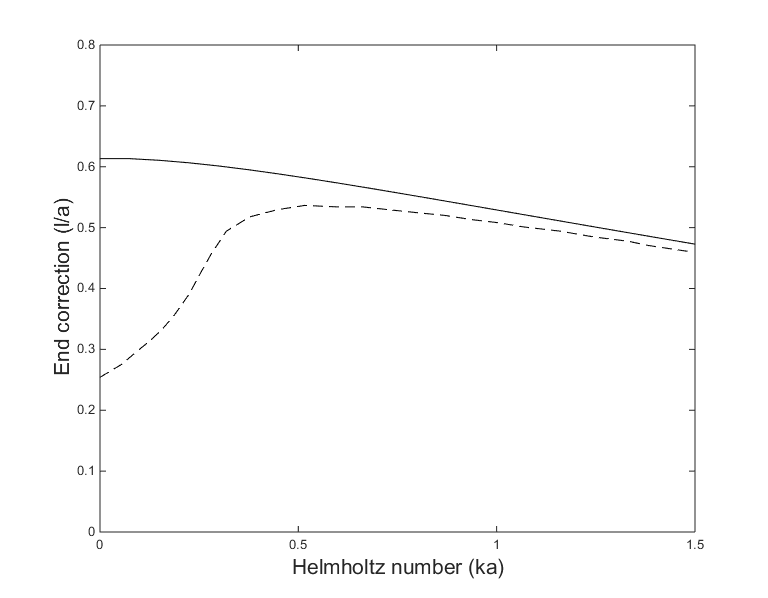
\includegraphics[width=.9\linewidth]{figuras/loa_comparacao.png}
  \caption[Coeficientes de correção de terminação $l/a$]{Resultados analíticos exatos para o coeficiente de correção da terminação normalizado pelo raio $l/a$ de um duto não flangeado. A linha contínua apresenta o resultado sem escoamento de \citeonline{levine1948radiation} e a linha tracejada apresenta o resultado com escoamento de Mach = 0,15 de \citeonline{munt1990acoustic}.}
  \label{fig:comp2}
\end{figure}
\newpage
De acordo com a Figura \ref{fig:comp2}, a correção normalizada da terminação $l/a$ torna-se consideravelmente menor do que aquela obtida na ausência de escoamento, sobretudo para baixos números de helmholtz ($ka$)\simbolo{$ka$}{Número de helmholtz}. Em outras palavras, para baixas frequências e na presença de um escoamento a onda acústica é refletida em uma região mais próxima da abertura, em comparação à situação sem escoamento.

No que diz respeito a modelos analíticos aproximados, o trabalho de \citeonline{carrier1955sound} foi um dos primeiros a abordar o cálculo do coeficiente de reflexão e correção da terminação com escoamento de exaustão num duto não flangeado. Para tal foi considerado um gás perfeito invíscido com o tipo de escoamento uniforme (\textit{plug}). Nessa abordagem usou-se a mesma metodologia que \citeonline{levine1948radiation} porém acoplando à formulação matemática o método de Prandtl-Glauert.

\citeonline{mani1973refraction} deu prosseguimento a mesma abordagem de \citeonline{carrier1955sound} com escoamento de exaustão, porém considerando a continuidade do deslocamento das partículas acústicas transversais. Esse tipo de solução mostra diversos fenômenos antes não previstos com os outros modelos citados como efeitos de convecção, zonas de silêncio relativo e refrações.

Também na mesma linha de desenvolvimento de \citeonline{carrier1955sound}, \citeonline{savkar1975radiation} desenvolveu um modelo de modos de alta ordem com escoamento de exaustão e sucção do tipo \texit{plug} com variação de temperatura. A continuidade do deslocamento das partículas acústicas transversais também foi considerada podendo também se passível de análise os fenômenos de convecção.



